\documentclass{article}
\usepackage{jcapstone}
\begin{document}

\section{Developing an Approximation}

Now that we have gotten to know our new distribution a little better, we can
use it to develop an approximation for the binomial.

Let $B \sim Bin(n, p)$ and $Y \sim SN(\mu, \sigma^2, \lambda)$. We will find
estimates for $\mu$, $\sigma$, and $\lambda$ by comparing the first, second,
and third moments about the mean of $B$ and $Y$.

\subsection{The Moments of the Binomial}

Let's start with the binomial. The first two moments are simply the mean and
variance, which we can state from memory:

\begin{equation*}
  E(B) = np, \quad Var(B) = np(1-p)
\end{equation*}

Having these, we can easily find

\begin{equation*}
  E(B^2) = Var(B) + [E(B)]^2 = np(1-p) + n^2p^2 = np - np^2 + n^2p^2
\end{equation*}

which we will need for the third moment. We will also need $E(B^3)$, which we
will get via the third factorial moment:

\begin{align*}
  E[B(B-1)(B-2)] &= \sum_{x=0}^n x (x-1) (x-2) \cdot \left\{ \binom{n}{x} p^x q^{n-x} \right\} \\
  \intertext{Notice that the first three terms of our sum are zero, so we can rewrite our sum beginning at $x = 3$:}
  &= \sum_{x=3}^n x(x-1)(x-2) \cdot \frac{n!}{x!\;(n-x)!} \; p^x q^{n-x} \\
  &= \sum_{x=3}^n \frac{n!}{(x-3)!\;(n-x)!} \; p^x q^{n-x} \\
  &= \sum_{x=3}^n n(n-1)(n-2) p^3 \cdot \frac{(n-3)!}{(x-3)!\;(n-x)!} \; p^{x-3}q^{n-x} \\
  \intertext{Let $y=x-3$. Then $x=y+3$, and $x=3, x=n \Ra y=0, y=n-3$.}
  &= n(n-1)(n-2)p^3 \cdot \sum_{y=0}^{n-3} \frac{(n-3)!}{y!\;(n-(y+3))!} \; p^y q^{n-(y+3)} \\
  &= n(n-1)(n-2)p^3 \cdot \underbrace {\sum_{y=0}^{n-3} \frac{(n-3)!}{y!\;((n-3)-y)!} \; p^y q^{(n-3)-y}}_{\mathclap{\textnormal{[pdf of $Bin(n-3,p)$ summed from 0 to $n-3$] = 1}}} \\
  &= n(n-1)(n-2)p^3 \\
  &= n^3p^3 - 3n^2p^3 + 2np^3 \\
  \intertext{Further expanding the left side and solving for $E(B^3)$,}
  E \left[ B^3 - 3B^2 + 2B \right] &= n^3p^3 - 3n^2p^3 + 2np^3 \\
  E(B^3) - 3E(B^2) + 2E(B) &= \\
  E(B^3) - 3(np - np^2 + n^2p^2) + 2np &= \\
  \Rightarrow \qquad E(B^3) &= n^3p^3 - 3n^2p^3 + 2np^3 + 3np - 3np^2 + 3n^2p^2 - 2np \\
  &= n^3p^3 - 3n^2p^3 + 2np^3 - 3np^2 + 3n^2p^2 + np
\end{align*}

Now, finally, we have all the building blocks necessary to obtain the third
moment:

\begin{align*}
  E \left( [B - E(B)]^3 \right) &= E \left( B^3 - 3B^2 E(B) + 3B [E(B)]^2 - [E(B)]^3 \right) \\
  &= E(B^3) - 3 E(B^2) E(B) + 3 E(B) [E(B)]^2 - [E(B)]^3 \\
  &= E(B^3) - 3 E(B^2) E(B) + 2 [E(B)]^3 \\
  &= (n^3p^3 - 3n^2p^3 + 2np^3 - 3np^2 + 3n^2p^2 + np) - 3(np - np^2 + n^2p^2)(np) + 2(np)^3 \\
  &= \cancel{n^3p^3} - \cancel{3n^2p^3} + 2np^3 - 3np^2 + \cancel{3n^2p^2} + np - \cancel{3n^2p^2} + \cancel{3n^2p^3} - \cancel{3n^3p^3} + \cancel{2n^3p^3} \\
  &= 2np^3 - 3np^2 + np \\
  &= np(p-1)(2p-1)
\end{align*}

Our hard-earned results, restated for convenience:

\begin{align}
  E(B) &= np \nonumber \\
  E([B - E(B)]^2) &= np(1-p) \\
  E([B - E(B)]^3) &= np(p-1)(2p-1) \nonumber
\end{align}

\subsection{The Moments of the Skew Normal}

Now we'll take a look at the moments of the skew normal. Equation
\eqref{eq:sn-basic-properties} takes care of the mean and variance; again the
third moment is a little more complicated:

\begin{align*}
  E([Y - E(Y)]^3) &= E(Y^3) - 3E(Y^2)E(Y) + 2[E(Y)]^3 \\
  &= (\mu^3 + 3 b \delta \mu^2 \sigma + 3 \mu \sigma^2 + 3 b \delta \sigma^3 - b \delta^3 \sigma^3) - 3 (\mu^2 + 2b \delta \mu \sigma + \sigma^2) (\mu + b \delta \sigma) \\
  & \quad + 2\;(\mu + b \delta \sigma)^3 \\
  &= \cancel{\mu^3} + \cancel{3 b \delta \mu^2 \sigma} + \cancel{3 \mu \sigma^2} + \cancel{3 b \delta \sigma^3} - b \delta^3 \sigma^3 - \cancel{3 \mu^3} - \cancel{3 b \delta \mu^2 \sigma} -
    \cancel{6 b \delta \mu^2 \sigma} - \cancel{6 b^2 \delta^2 \mu \sigma^2} - \cancel{3 \mu \sigma^2} \\
  & \quad - \cancel{3 b \delta \sigma^3} + \cancel{2 \mu^3} + \cancel{6 b \delta \mu^2 \sigma} + \cancel{6 b^2 \delta^2 \mu \sigma^2} + 2 b^3 \delta^3 \sigma^3 \\
  &= 2 b^3 \delta^3 \sigma^3 - b \delta^3 \sigma^3 \\
  &= b \delta^3 \sigma^3 (2b^2 - 1)
\end{align*}

We restate our results:

\begin{alignat}{4}
  E(Y) &= \mu + b \delta \sigma \;&=&\; \mu + \sigma \cdot \sqrt{\frac{2}{\pi}} \cdot \frac{\lambda}{\sqrt{1 + \lambda^2}} \nonumber \\
  E([Y - E(Y)]^2) &= \sigma^2 (1 - b^2 \delta^2) \;&=&\; \sigma^2 \left( 1 - \frac{2}{\pi} \cdot \frac{\lambda^2}{1 + \lambda^2} \right) \\
  E([Y - E(Y)]^3) &= b \delta^3 \sigma^3 (2b^2 - 1) \;&=&\; \sigma^3 \sqrt{\frac{2}{\pi}} \left( \frac{\lambda}{\sqrt{1 + \lambda^2}} \right)^3 \left( \frac{4}{\pi} - 1 \right) \nonumber
\end{alignat}

\subsection{Solving for $\mu$, $\sigma$, $\lambda$}

Now we can set the moments of our two distributions equal to each other and,
taking $n$ and $p$ as constants, solve for $\mu$, $\sigma$ and $\lambda$.

\begin{subequations}
\begin{align}
  np &= \mu + \sigma \cdot \sqrt{\frac{2}{\pi}} \cdot \frac{\lambda}{\sqrt{1 + \lambda^2}} \label{eq:first-moment-set} \\
  np(1-p) &= \sigma^2 \left( 1 - \frac{2}{\pi} \cdot \frac{\lambda^2}{1 + \lambda^2} \right) \label{eq:second-moment-set} \\
  np(p-1)(2p-1) &= \sigma^3 \sqrt{\frac{2}{\pi}} \left( \frac{\lambda}{\sqrt{1 + \lambda^2}} \right)^3 \left( \frac{4}{\pi} - 1 \right) \label{eq:third-moment-set}
\end{align}
\end{subequations}

To get $\lambda$, we divide the cube of \eqref{eq:second-moment-set} by the
square of \eqref{eq:third-moment-set}:

\begin{align}
  \frac{\sigma^6 \left( 1 - \frac{2}{\pi} \cdot \frac{\lambda^2}{1 + \lambda^2} \right)^3}{\sigma^6 \cdot \frac{2}{\pi} \left( \frac{\lambda}{\sqrt{1 + \lambda^2}} \right)^6 \left(
    \frac{4}{\pi} - 1 \right)^2} &= \frac{n^3p^3(1-p)^3}{n^2p^2(p-1)^2(2p-1)^2} \nonumber \\
  \Rightarrow \quad \frac{\left( 1 - \frac{2}{\pi} \cdot \frac{\lambda^2}{1+\lambda^2} \right)^3}{\frac{2}{\pi} \left( \frac{\lambda^2}{1+\lambda^2} \right)^3 \left( \frac{4}{\pi} - 1
    \right)^2} &= \frac{np(1-p)}{(1-2p)^2} \label{eq:solving-for-lambda}
\end{align}

The above equation \eqref{eq:solving-for-lambda} is a rational expression in
$\lambda^2$ that can be solved with either a considerable amount of manual
labor or, more efficiently, with a computer algebra system. Once we have
$\lambda^2$, then $\lambda$ is simply either the positive or negative square
root, as determined by the sign of $(1-2p)$. This can be explained with a
little assistance from Property \ref{prop:3}: When $p \to 0$, the binomial
skews left and converges toward the positive half normal, which by
\eqref{eq:p2-positive-half-normal} corresponds to a positive $\lambda$. When $p
\to 1$, the binomial skews right and converges toward the negative half normal,
which by \eqref{eq:p2-negative-half-normal} corresponds to a negative
$\lambda$. When $p = 0.5$, the binomial is symmetric and $\lambda$ is 0,
eliminating the need for a sign. Thus:

\begin{equation}
  \label{eq:lambda-solved}
  \lambda = \textnormal{\{sign of $(1-2p)$\}} \sqrt{\lambda^2}
\end{equation}

Having secured $\lambda$, we can find $\sigma$ using
\eqref{eq:second-moment-set}:

\begin{equation}
  \label{eq:sigma-solved}
  np(1-p) = \sigma^2 \left( 1 - \frac{2}{\pi} \cdot \frac{\lambda^2}{1 + \lambda^2} \right) \quad\Rightarrow\quad
  \sigma = \sqrt{\frac{np(1-p)}{1 - \frac{2}{\pi} \cdot \frac{\lambda^2}{1 + \lambda^2}}}
\end{equation}

And with both $\lambda$ and $\sigma$, a simple rearrangement of
\eqref{eq:first-moment-set} yields $\mu$:

\begin{equation}
  \label{eq:mu-solved}
  np = \mu + \sigma \cdot \sqrt{\frac{2}{\pi}} \cdot \frac{\lambda}{\sqrt{1 + \lambda^2}} \quad\Rightarrow\quad
  \mu = np - \sigma \cdot \sqrt{\frac{2}{\pi}} \cdot \frac{\lambda}{\sqrt{1 + \lambda^2}}
\end{equation}

When $p = 0.5$, we would expect the binomial to be perfectly symmetrical and
therefore $\mu = np = n/2$. From \eqref{eq:mu-solved}, this implies that
$\sigma \cdot \sqrt{\frac{2}{\pi}} \cdot \frac{\lambda}{\sqrt{1 + \lambda^2}} =
0 \Ra$ either $\sigma = 0$ or $\lambda = 0$. Since the former is impossible, we
must conclude the latter, which brings us back to the normal distribution.

\subsection{Restrictions}

To obtain an estimate for $\lambda$, we must put a few restrictions on $n$ and
$p$.

If we let $u = \frac{\lambda^2}{1+\lambda^2}$ and $v = 1/u$, we can rewrite the
left hand side of \eqref{eq:solving-for-lambda} as

\begin{alignat*}{3}
  \frac{\left( 1 - \frac{2}{\pi} \cdot \frac{\lambda^2}{1+\lambda^2} \right)^3}{\frac{2}{\pi} \left( \frac{\lambda^2}{1+\lambda^2} \right)^3 \left( \frac{4}{\pi} - 1 \right)^2}
    &= \left. \left( 1 - \frac{2}{\pi} u \right)^3 \middle/ \frac{2}{\pi} u^3 \left( \frac{4}{\pi} - 1 \right)^2 \right. & \\
  &= \left( 1 - \frac{2}{\pi} u \right)^3 \cdot v^3 \cdot \frac{\pi}{2} \cdot \left( \frac{\pi}{4-\pi} \right)^2 & \\
  &= \left[ v \left( 1 - \frac{2}{\pi} u \right) \right]^3 \left( \frac{\pi^3}{2(4-\pi)^2} \right) & \\
  &= \left( v - \frac{2}{\pi} \right)^3 \left( \frac{\pi^3}{2(4-\pi)^2} \right) &= g(v).
\end{alignat*}

We can see that $g(v)$ is increasing in $v$, which is always $\geq 1$.
Therefore:

\begin{equation}
  \min_{v} g(v) = g(v)|_{v=1} = \left( 1 - \frac{2}{\pi} \right)^3 \left( \frac{\pi^3}{2(4-\pi)^2} \right) = 1.009524 \approx 1,
\end{equation}

which means that the right hand side of \eqref{eq:solving-for-lambda}, which is
supposed to be equal to the left hand side of \eqref{eq:solving-for-lambda},
can't ever be less than 1. Unfortunately, it sometimes is; in particular,
$\frac{np(1-p)}{(1-2p)^2} \to 0$ when $p \to 0$ or $p \to 1$. So if we want a
solution, we must restrict $n$ and $p$ such that

\begin{align}
  \textnormal{\{right hand side of \eqref{eq:solving-for-lambda}\}} &\geq \textnormal{\{min of left hand side of \eqref{eq:solving-for-lambda}\}} \nonumber \\
  \frac{np(1-p)}{(1-2p)^2} &\geq 1 \nonumber \\
  np(1-p) &\geq (1-2p)^2 \label{eq:solving-the-restriction}
\end{align}

Here, two scenarios arise. The first is when we have a fixed $p$ and wish to
find the minimum $n$ necessary to derive a skew-normal approximation. From
\eqref{eq:solving-the-restriction}, this is very simple:

\begin{equation}
  n \geq \frac{(1-2p)^2}{p(1-p)} \label{eq: n for a given p}
\end{equation}

Figure \ref{fig:sn-restriction-least-n} shows the least sample size required to
estimate $\lambda$ as a function of $p$. As expected, it is quite large when
$p$ is small and rapidly goes to 0 as $p$ increases; for example, when $p =
0.01$, $n$ must be $\geq 98$, but at $p = 0.2$, $n$ need only be $\geq 3$, a
trivial requirement to meet.

\begin{figure}
  \centering
  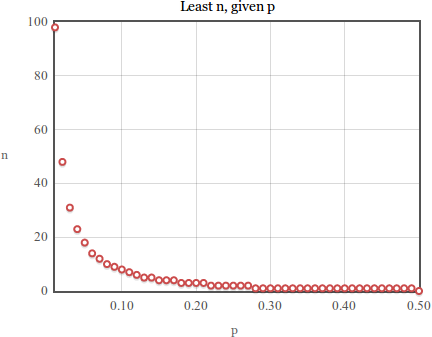
\includegraphics[width=0.6\textwidth]{../graphs/images/restriction-least-n.png}
  \caption{Least possible $n$, given a fixed $p$}
  \label{fig:sn-restriction-least-n}
\end{figure}

The second scenario is when $n$ is fixed and we wish to solve for $p$. In this
case, we return to \eqref{eq:solving-the-restriction} for further factoring:

\begin{align}
  np - np^2 &\geq 1 - 4p + 4p^2 \nonumber \\
  1 - 4p + 4p^2 - np + np^2 &\leq 0 \nonumber \\
  (n+4)p^2 - (n+4)p + 1 &\leq 0 \label{eq: solving for p}
\end{align}

We then apply the quadratic formula with $a = n+4$, $b = -(n+4)$, and $c = 1$:

\begin{align*}
  p &= \frac{(n+4) \pm \sqrt{(n+4)^2 - 4 \cdot (n+4) \cdot 1}}{2(n+4)} \\
  &= \frac{(n+4) \pm \sqrt{n^2 + 8n + 16 - 4n - 16}}{2(n+4)} \\
  &= \frac{(n+4) \pm \sqrt{n^2 + 4n}}{2(n+4)} \\
  &= \frac{n+4}{2(n+4)} \pm \frac12 \sqrt{\frac{n(n+4)}{(n+4)^2}} \\
  &= \frac12 \pm \frac12 \sqrt{\frac{n}{n+4}}
\end{align*}

Let $r_1 = \frac12 - \frac12 \sqrt{\frac{n}{n+4}}$ and $r_2 = \frac12 + \frac12
\sqrt{\frac{n}{n+4}}$. (Note that $r_1 < r_2$.) Now we can rewrite \eqref{eq:
solving for p} as

\begin{equation*}
  (p - r_1)(p - r_2) \leq 0
\end{equation*}

Examining the left hand side, when $p < r_1$, both terms are negative and so
their product is positive; when $p > r_2$, both terms are positive, again
leading the product to be positive. Therefore, our solution lies where $r_1
\leq p \leq r_2$, or more explicitly:

\begin{equation}
 \frac12 - \frac12 \sqrt{\frac{n}{n+4}} \; \leq \; p \; \leq \; \frac12 + \frac12 \sqrt{\frac{n}{n+4}}
\end{equation}

Shown in figure \ref{fig:sn-restriction-p-range} as a function of $n$, this
interval grows quickly as $n$ increases, and for sufficiently large $n$, it
becomes almost $(0, 1)$. For example, when $n=100$, our interval is $(0.00971,
0.99029)$; when $n=500$, it is (0.00199, 0.99801).

\begin{figure}
  \centering
  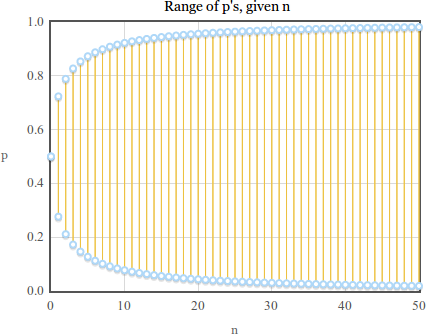
\includegraphics[width=0.6\textwidth]{../graphs/images/restriction-p-range.png}
  \caption{Range of possible $p$, given a fixed $n$}
  \label{fig:sn-restriction-p-range}
\end{figure}

For those unfortunate combinations of $n$ and $p$ so extreme that our
skew-normal approximation will not work, our authors suggest a Poission
approximation.

\appendix
\section{Solving for $\lambda$}
\label{sec:solving-for-lambda}

Hoping that it would provide some insight into \eqref{eq:lambda-solved}, I
expanded \eqref{eq:solving-for-lambda} after moving all terms to the left hand
side:

\begin{gather*}
  \left. \left( 1 - \frac{2}{\pi} \cdot \frac{\lambda^2}{1+\lambda^2} \right)^3 \middle/ \left[ \frac{2}{\pi} \left( \frac{\lambda^2}{1+\lambda^2} \right)^3 \left( \frac{4}{\pi} - 1
    \right)^2 \right] \right. \;-\; \frac{np(1-p)}{(1-2p)^2} \\
  \left. \left( \frac{\pi(1+\lambda^2) - 2\lambda^2}{\pi(1+\lambda^2)} \right)^3 \middle/ \left( \frac{2(4-\pi)^2\lambda^6} {\pi^3(1+\lambda^2)^3} \right) \right. \;-\; \frac{np(1-p)}{(1-2p)^2} \\
  \left( \frac{\pi^3(1+\lambda^2)^3 - 3\pi^2(1+\lambda^2)^2 \cdot 2\lambda^2 + 3\pi(1+\lambda^2) \cdot 4\lambda^4 - 8\lambda^6}{\cancel{\pi^3 (1+\lambda^2)^3}} \right) \cdot \left(
    \frac{\cancel{\pi^3(1+\lambda^2)^3}}{2(4-\pi)^2\lambda^6} \right) \;-\; \frac{np(1-p)}{(1-2p)^2} \\
  \frac{\pi^3(1+3\lambda^2+3\lambda^4+\lambda^6) - 6\pi^2\lambda^2(1+2\lambda^2+4\lambda^4) + 12\pi\lambda^4(1+\lambda^2) - 8\lambda^6}{2(4-\pi)^2\lambda^6} \;-\; \frac{np(1-p)}{(1-2p)^2} \\
  \frac{\pi^3 + 3\pi^3\lambda^2 + 3\pi^3\lambda^4 + \pi^3\lambda^6 - 6\pi^2\lambda^2 - 12\pi^2\lambda^4 - 24\pi^2\lambda^6 + 12\pi\lambda^4 + 12\pi\lambda^6 - 8\lambda^6}{2(4-\pi)^2\lambda^6}
    \;-\; \frac{np(1-p)}{(1-2p)^2} \\
  \frac{\lambda^6(\pi^3-24\pi^2+12\pi-8) + \lambda^4(3\pi^3-12\pi^2+12\pi) + \lambda^2(3\pi^3-6\pi^2) + \pi^3}{2(4-\pi)^2\lambda^6} \;-\; \frac{np(1-p)}{(1-2p)^2}
  \intertext{Taking $c_1 = \pi^3 - 24\pi^2 + 12\pi - 8$, $c_2 = 3\pi^3 - 12\pi^2 + 12\pi$, $c_3 = 3\pi^3 - 6\pi^2$, $c_4 = \pi^3$, and $c_5 = 2(4-\pi)^2$, we can simplify this to}
  \frac{c_1\lambda^6 + c_2\lambda^4 + c_3\lambda^2 + c_4}{c_5\lambda^6} - \frac{np(1-p)}{(1-2p)^2} \\
  \frac{c_1(1-2p)^2\lambda^6 + c_2(1-2p)^2\lambda^4 + c_3(1-2p)^2\lambda^2 + c_4(1-2p)^2 - c_5\;np(1-p)\lambda^6}{c_5(1-2p)^2\lambda^6} \\
  \frac{\left[c_1(1-2p)^2 - c_5\;np(1-p)\right]\lambda^6 + \left[c_2(1-2p)^2\right]\lambda^4 + \left[c_3(1-2p)^2\right]\lambda^2 + c_4(1-2p)^2}{c_5(1-2p)^2\;\lambda^6}
\end{gather*}

\section{Curiosity}

As a curiosity, I was unable to get Pewsey and Azzalini to agree with each
other on $E(Z^3)$. According to Pewsey (2000),

\begin{equation} \label{eq:ey3-pewsey}
  E(Y^3) = \mu^3 + 3 b \delta \mu^2 \sigma + 3 \mu \sigma^2 + 3 b \delta \sigma^3 - b \delta^3 \sigma^3
\end{equation}

where $b = \sqrt{\frac{2}{\pi}}$ and $\delta = \frac{\lambda}{\sqrt{1 +
\lambda^2}} \in (-1, 1)$. Since $Y = \mu + \sigma Z$, by the linearity of
expected value, we also have

\begin{align}
  E(Y^3) &= E \left[ (\mu + \sigma Z)^3 \right] \nonumber \\
  &= E (\mu^3 + 3 \mu^2 \sigma Z + 3 \mu \sigma^2 Z^2 + \sigma^3 Z^3) \nonumber \\
  &= \mu^3 + 3 \mu^2 \sigma\;E(Z) + 3 \mu \sigma^2\;E(Z^2) + \sigma^3\;E(Z^3) \nonumber \\
  &= \mu^3 + 3 b \delta \mu^2 \sigma + 3 \mu \sigma^2 + \sigma^3\;E(Z^3) \label{eq:ey3-linear-expansion}
\end{align}

By comparing equations \eqref{eq:ey3-pewsey} and
\eqref{eq:ey3-linear-expansion} and eliminating terms, we arrive at

\begin{align}
  \sigma^3\;E(Z^3) &= 3 b \delta \sigma^3 - b \delta^3 \sigma^3 \nonumber \\
  \Rightarrow \quad E(Z^3) &= 3 b \delta - b \delta^3 \nonumber \\
  &= b \delta (3 - \delta^2) \nonumber \\
  &= \sqrt{\frac{2}{\pi}} \cdot \frac{\lambda}{\sqrt{1 + \lambda^2}} \cdot \left( 3 - \frac{\lambda^2}{1 + \lambda^2} \right) \label{eq:ez3-pewsey-derived}
\end{align}

However, according to equation (6.5?) in Azzalini (2005),

\begin{equation}
  E(Z^r) =
  \begin{dcases*}
    1 \times 3 \times \cdots \times (r -1) & if r is even \\
    \frac{\sqrt{2}\;(2k + 1)!\;\lambda}{\sqrt{\pi}\;(1 + \lambda^2)^{k + 1/2}\;2^k} \sum_{m=0}^k\;\frac{m!\;(2\lambda)^{2m}}{(2m+1)!\;(k-m)!} & if $r = 2k+1$ and $k = 0, 1, ...$
  \end{dcases*}
\end{equation}

So, for $E(Z^3)$, we have $r = 2k + 1 = 3$ and $k = 1$:

\begin{align}
  E(Z^3) &= \frac{\sqrt{2} \cdot 3! \cdot \lambda}{\sqrt{\pi} \cdot (1 + \lambda^2)^{3/2} \cdot 2} \; \sum_{m=0}^1 \frac{m!\;(2\lambda)^{2m}}{(2m + 1)!\;(1 - m)!} \nonumber \\
  &= \frac{3\sqrt{2}}{\sqrt{\pi}} \cdot \frac{\lambda}{(1 + \lambda^2)^{3/2}} \cdot \left( \frac{0! (2\lambda)^0}{1!1!} + \frac{1! (2\lambda)^2}{3!0!} \right) \nonumber \\
  &= \frac{3\sqrt{2}}{\sqrt{\pi}} \cdot \frac{\lambda}{(1 + \lambda^2)^{3/2}} \cdot \left( 1 + \frac{2}{3}\lambda^2 \right) \nonumber \\
  &= \sqrt{\frac{2}{\pi}} \cdot \frac{\lambda}{(\sqrt{1 + \lambda^2})^3} \cdot (3 + 2 \lambda^2) \label{eq:ez3-azzalini}
\end{align}

Unfortunately, equations \eqref{eq:ez3-pewsey-derived} and
\eqref{eq:ez3-azzalini} do not really line up.

\bibliography{/home/joycetipping/projects/capstone/pieces/bibliography/bibliography.bib}
\bibliographystyle{plainnat}
\end{document}
